\documentclass{zpt}
\title{实验一}
\begin{document}
    \maketitle
    \tableofcontents
    \section{实验内容}
    用C++实现对C--语言的词法分析器。
    \section{程序设计原理与方法}
    \subsection{原理}
    在教材上给出了C--语言的部分单词类型的有限状态自动机, 老师给出了更健全的正则表达式, 对两者进行分析, 结合有限状态自动机, 以老师给出的伪代码为框架, 自己实现词法分析器。
    \subsection{方法}
    在明确了各个组成成为的正则表达式后, 利用C++的$\mathrm{if, else}$语句, $\mathrm{switch,case}$语句实现状态之间的切换, 同时处理各种错误。\par
    \textbf{需要注意的, 词法分析器不涉及语法语义的处理, 所有要做的事情可以抽象为下面的流程图:}
    \begin{figure}[H]
        \centering
        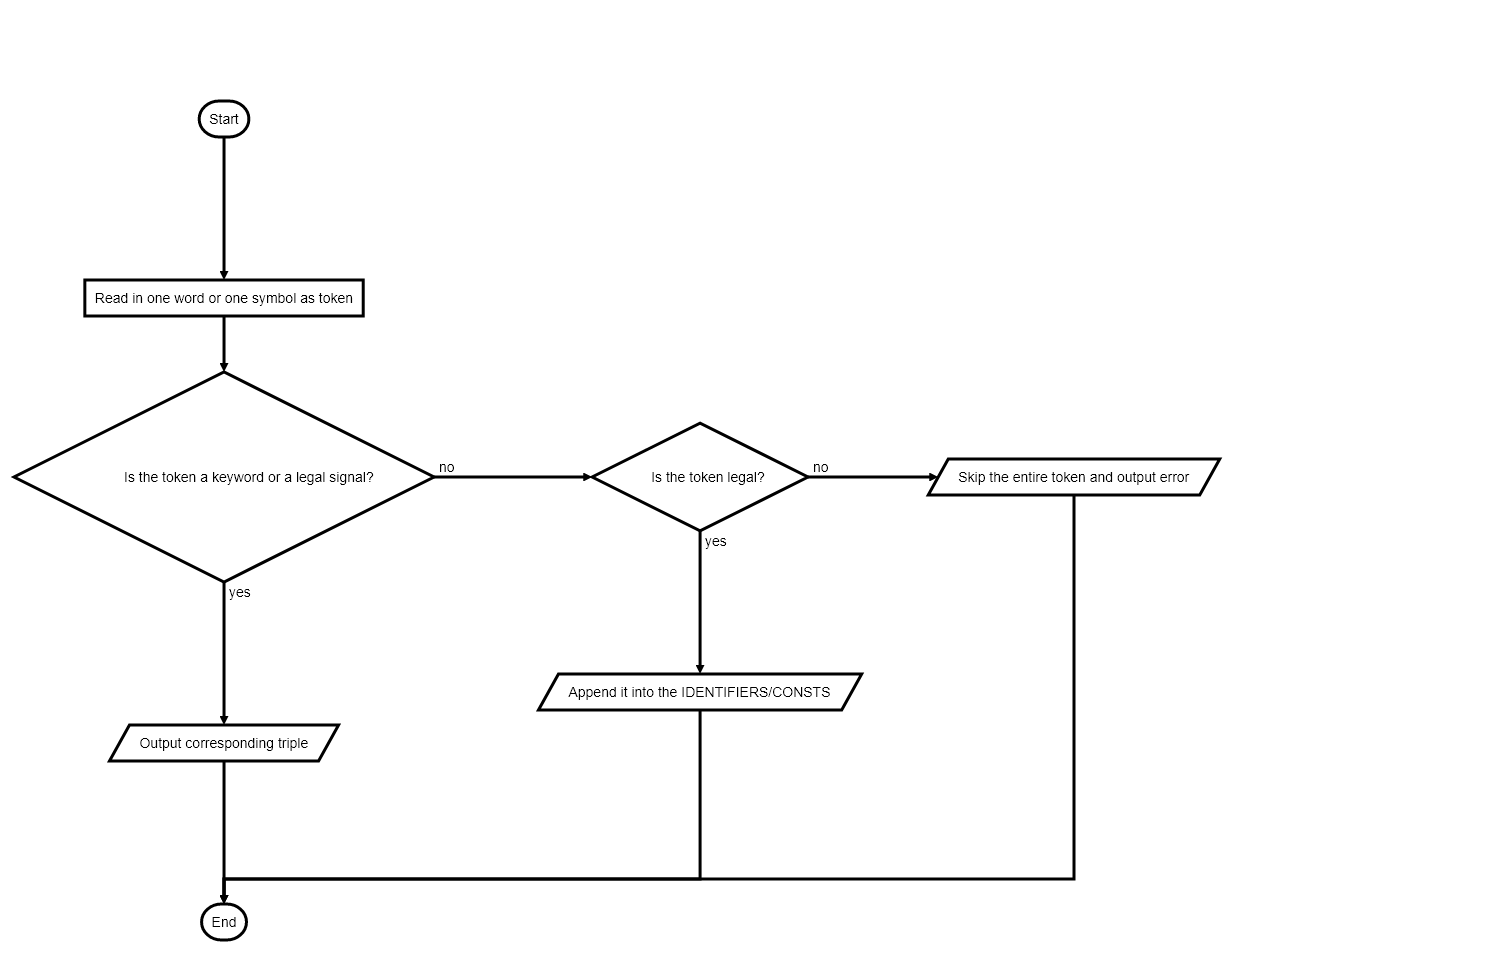
\includegraphics[width=\textwidth]{flowchart.png}
    \end{figure}
    因此程序需要做的变得很简单, 即通过一个while循环连续地读入token之后处理token即可。
    \section{程序设计流程}
    根据上一个section, 我们可以直观地讲词法分析器抽象成如下格式:

    \begin{algorithm}[H]
        \While{getchar()}{
            \uIf{word}{
                parse\_keywords\_and\_identifiers();
            }
            \uElseIf{digit}{
                parse\_digit();
            }
            \uElseIf{operator}{
                parse\_operator();\\
                \uIf{$//$}{
                    parse\_comment\_line();
                }
                \uElseIf{$/*$}{
                    parse\_comment\_block();
                }
            }
            \uElseIf{separator}{
                parse\_separator();
            }
            \Else{
                parse\_error();
            }
        }
        \caption{Lexer}
    \end{algorithm}
    在每个parse\_xxx的函数中进行判断是否读到了当前token的结束, 以及输出和最后对已读取token的清除。
    \section{程序设计清单}
    如上, 我们要设计实现\textbf{七种parse function};除此之外, 由于我\textbf{预先将keywords, operator和separator都存放在分别的文件里, 需要设计相应的utility function来进行加载}, 并且需要封装读取字符功能以及输出功能。\par
    我使用std::map来保存一系列预先定义/代码生成的表, 包括预先定义的Keywords, Operators, Separators, 和代码生成的Identifiers, Consts;对于所有字典, 我将token作为字典的键, 将其在该字典中的序号作为对应的值;同时分别写入文件, 使用\\t作为分隔符, 每一个token占一行。
    \section{运行结果}
    对lexer.cpp进行词法分析, \emph{即将源代码作为输入文件}, 得到结果部分展示如\reff{f1}:
    \begin{figure}
        \centering
        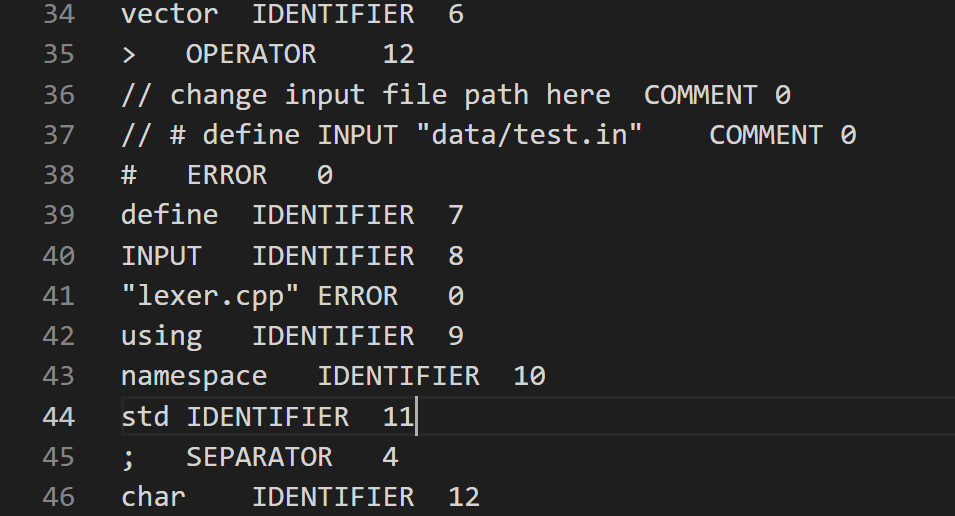
\includegraphics[width=7cm]{result.png}
        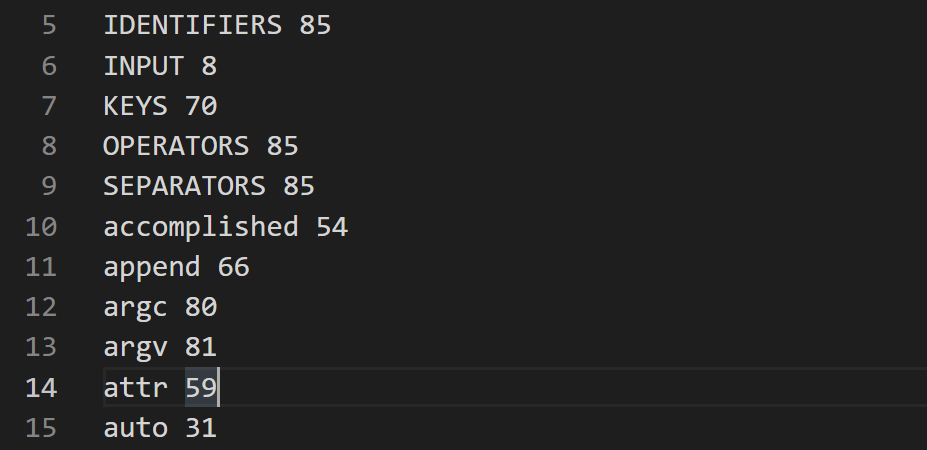
\includegraphics[width=7cm]{identifiers.png}
        \caption{result(左), identifier(右)}
        \label{f1}
    \end{figure}
    \section{程序使用说明}
    \begin{enumerate}
        \item 在data/KeyWords.txt中修改预设关键词;
        \item 在data/Operators.txt中修改预设操作符;
        \item 在data/Separators.txt中修改预设分隔符;
        \item 在lexer.cpp的宏定义中修改INPUT为测试文件路径, 即可编译运行;
        \item \emph{最后默认会将每个词的分析结果写入result.txt, 并将identifier写入identifiers.txt, 将consts写入consts.txt。}
    \end{enumerate}
    \section{总结与完善}
    \begin{itemize}
    \item 之前由于没有分清楚词法分析和语法分析, 纠结了很长时间, 后来才理清逻辑。
    \item 在解析(\emph{尤其是小数})的时候, 很难按照有限状态自动机的逻辑去处理, 只能判断一些条件看是否报错, 和师兄交流过是否有更好的逻辑, 发现难以做到。
    \end{itemize}
\end{document}